\documentclass{article}
\usepackage{graphicx}
\usepackage{float}
\usepackage{subcaption}

\begin{document}
\title{Study of two Raspberry Pis and Power adapters}
\author{Abhinav Narain}
\maketitle
\section{Raspberry Pi and Power Adapters}
Two raspberry pis and two adapters and two power-cables were used for
measuring EMI on channel and the document shows how the EMI generated
is distinct to the extent, that one~\ref{fig:r1} doesn't produce any
EMI while other one~\ref{fig:r2} does.

\begin{enumerate}
\item Raspberry Pi Model B $+$ V1.2 (Fig~\ref{fig:r1})
\item Raspberry Pi 3 Model BV1.2 (Fig~\ref{fig:r2})
\end{enumerate}

\begin{enumerate}
\item Powerchord 1 (Fig ~\ref{fig:p1}) using a USB cable
\item Powerchord 2 (Fig ~\ref{fig:p2}) usual usual cable (non-USB) 
\end{enumerate}

\subsection{Compare EMI of two power adapters}
\begin{figure}[H]
  \centering
  \begin{subfigure}{\textwidth}
    \centering
    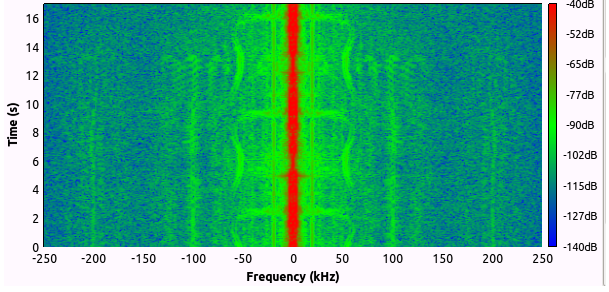
\includegraphics[width=\textwidth]{./figures/raspi-with-usb.png}
    \vspace{-25pt}
    \caption{EMI generated by Raspberry Pi with USB power chord (1)}
    \label{fig:u0}
  \end{subfigure}
  \begin{subfigure}{\textwidth}
    \centering
    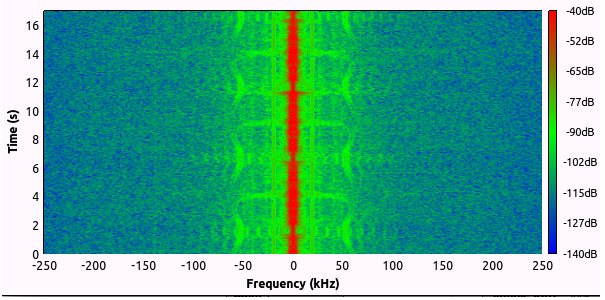
\includegraphics[width=\textwidth]{./figures/raspi-without-usb.png}
    \caption{EMI generated by Raspberry Pi with different power-chord (2)}
    \label{fig:u1}
  \end{subfigure}
  \caption{Same Raspberry Pi-2 shows two different EMI signatures for two different power-chords}
  \label{fig:u2}
\end{figure}

\subsection{Compare EMI of two Raspberry Pis}
\begin{figure}[H]
  \centering
  \begin{subfigure}{\textwidth}
    \centering
    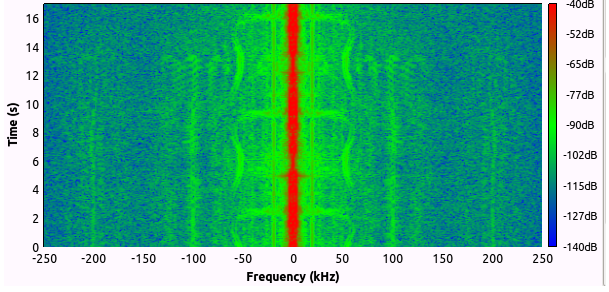
\includegraphics[width=\textwidth]{./figures/raspi-with-usb.png}
    \vspace{-25pt}
    \caption{EMI generated by Raspberry 2 with USB power chord (1)}
    \label{fig:g0}
  \end{subfigure}
  
    \begin{subfigure}{\textwidth}
      \centering
      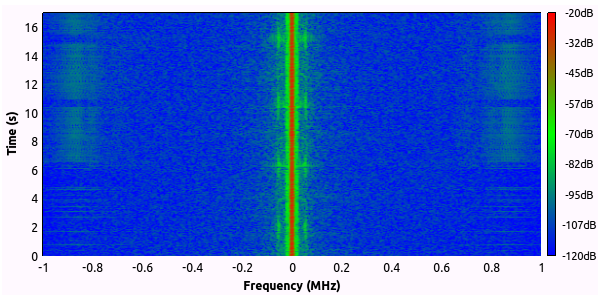
\includegraphics[width=\textwidth]{./figures/raspi-old.png}
      \caption{EMI generated by Raspberry 1 with USB power chord (1)}
      \label{fig:g1}
    \end{subfigure}
    \caption{Two different Raspberry Pi using the same power chord but have different EMI signatures }
    \label{fig:g2}
\end{figure}

\section{Miscellaneous}
The Raspberry Pis are shown below
\begin{figure*}[t]
  \centering
  \begin{subfigure}{.5\textwidth}
  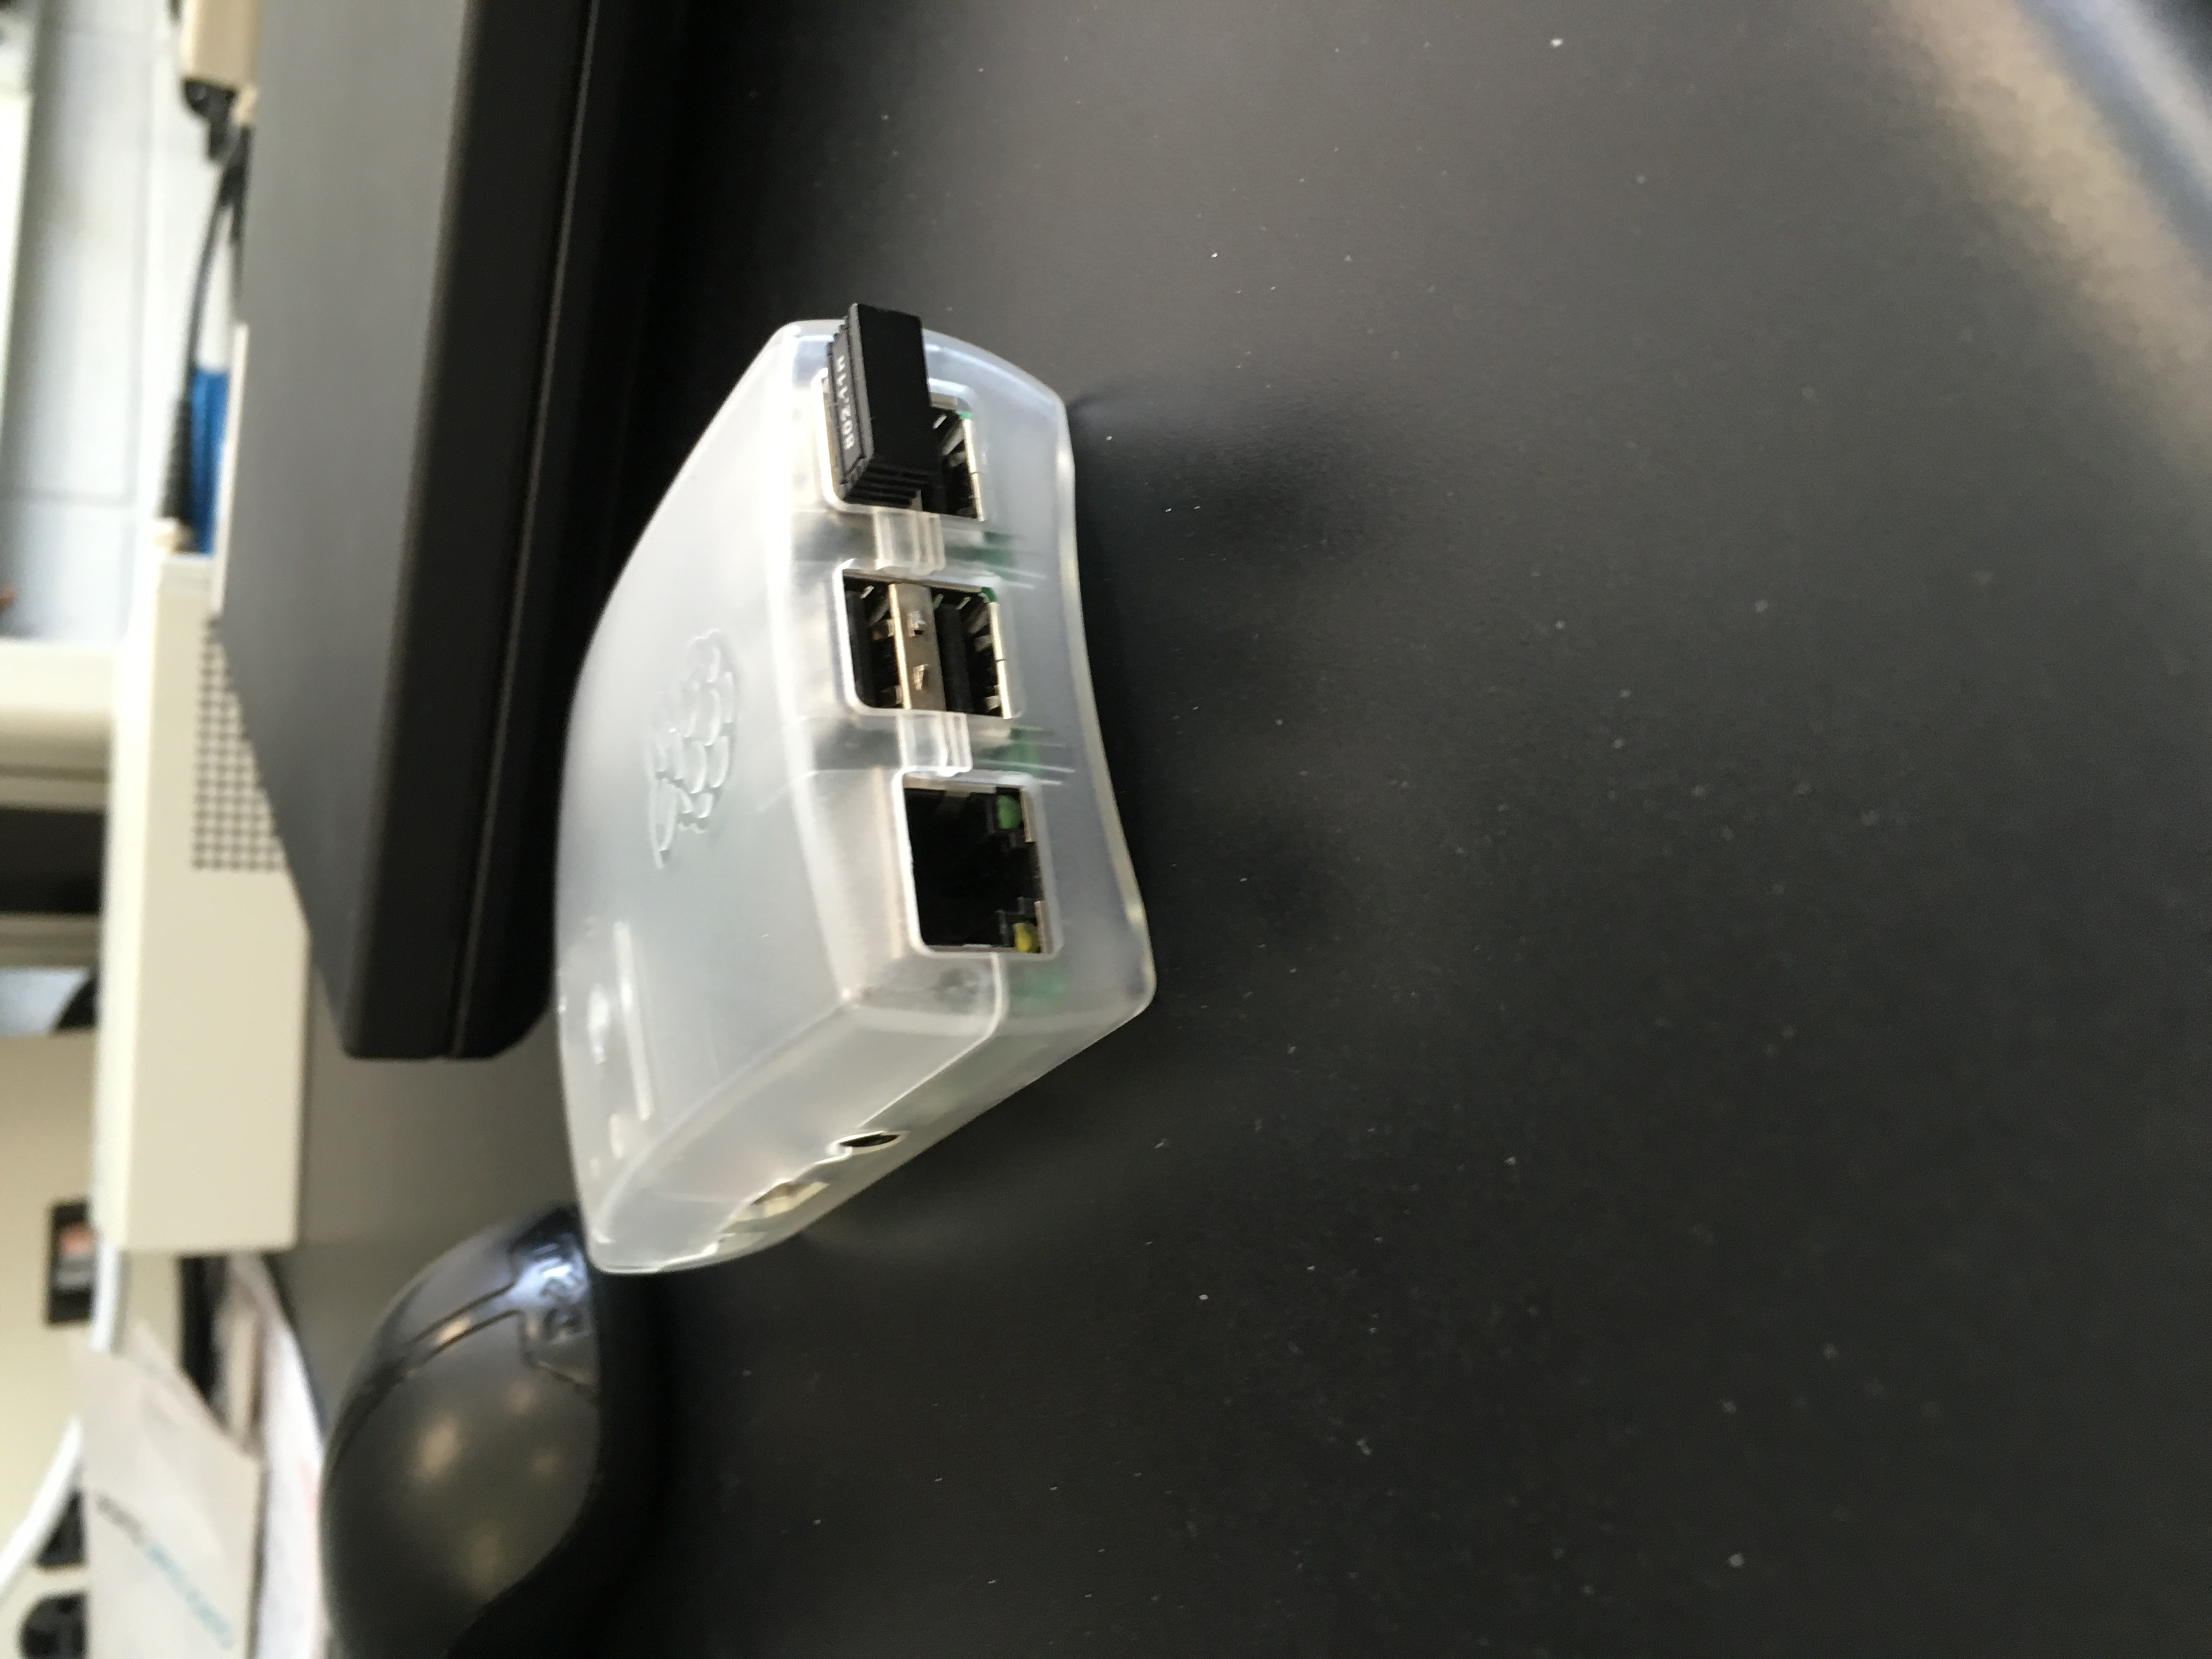
\includegraphics[width=\textwidth]{./figures//IMG_0709.JPG}
  \caption{Raspberry 1 (Raspberry Pi) }
  \label{fig:r1}
  \end{subfigure}\hfill% 
  \centering
  \begin{subfigure}{.5\textwidth}
    \centering
    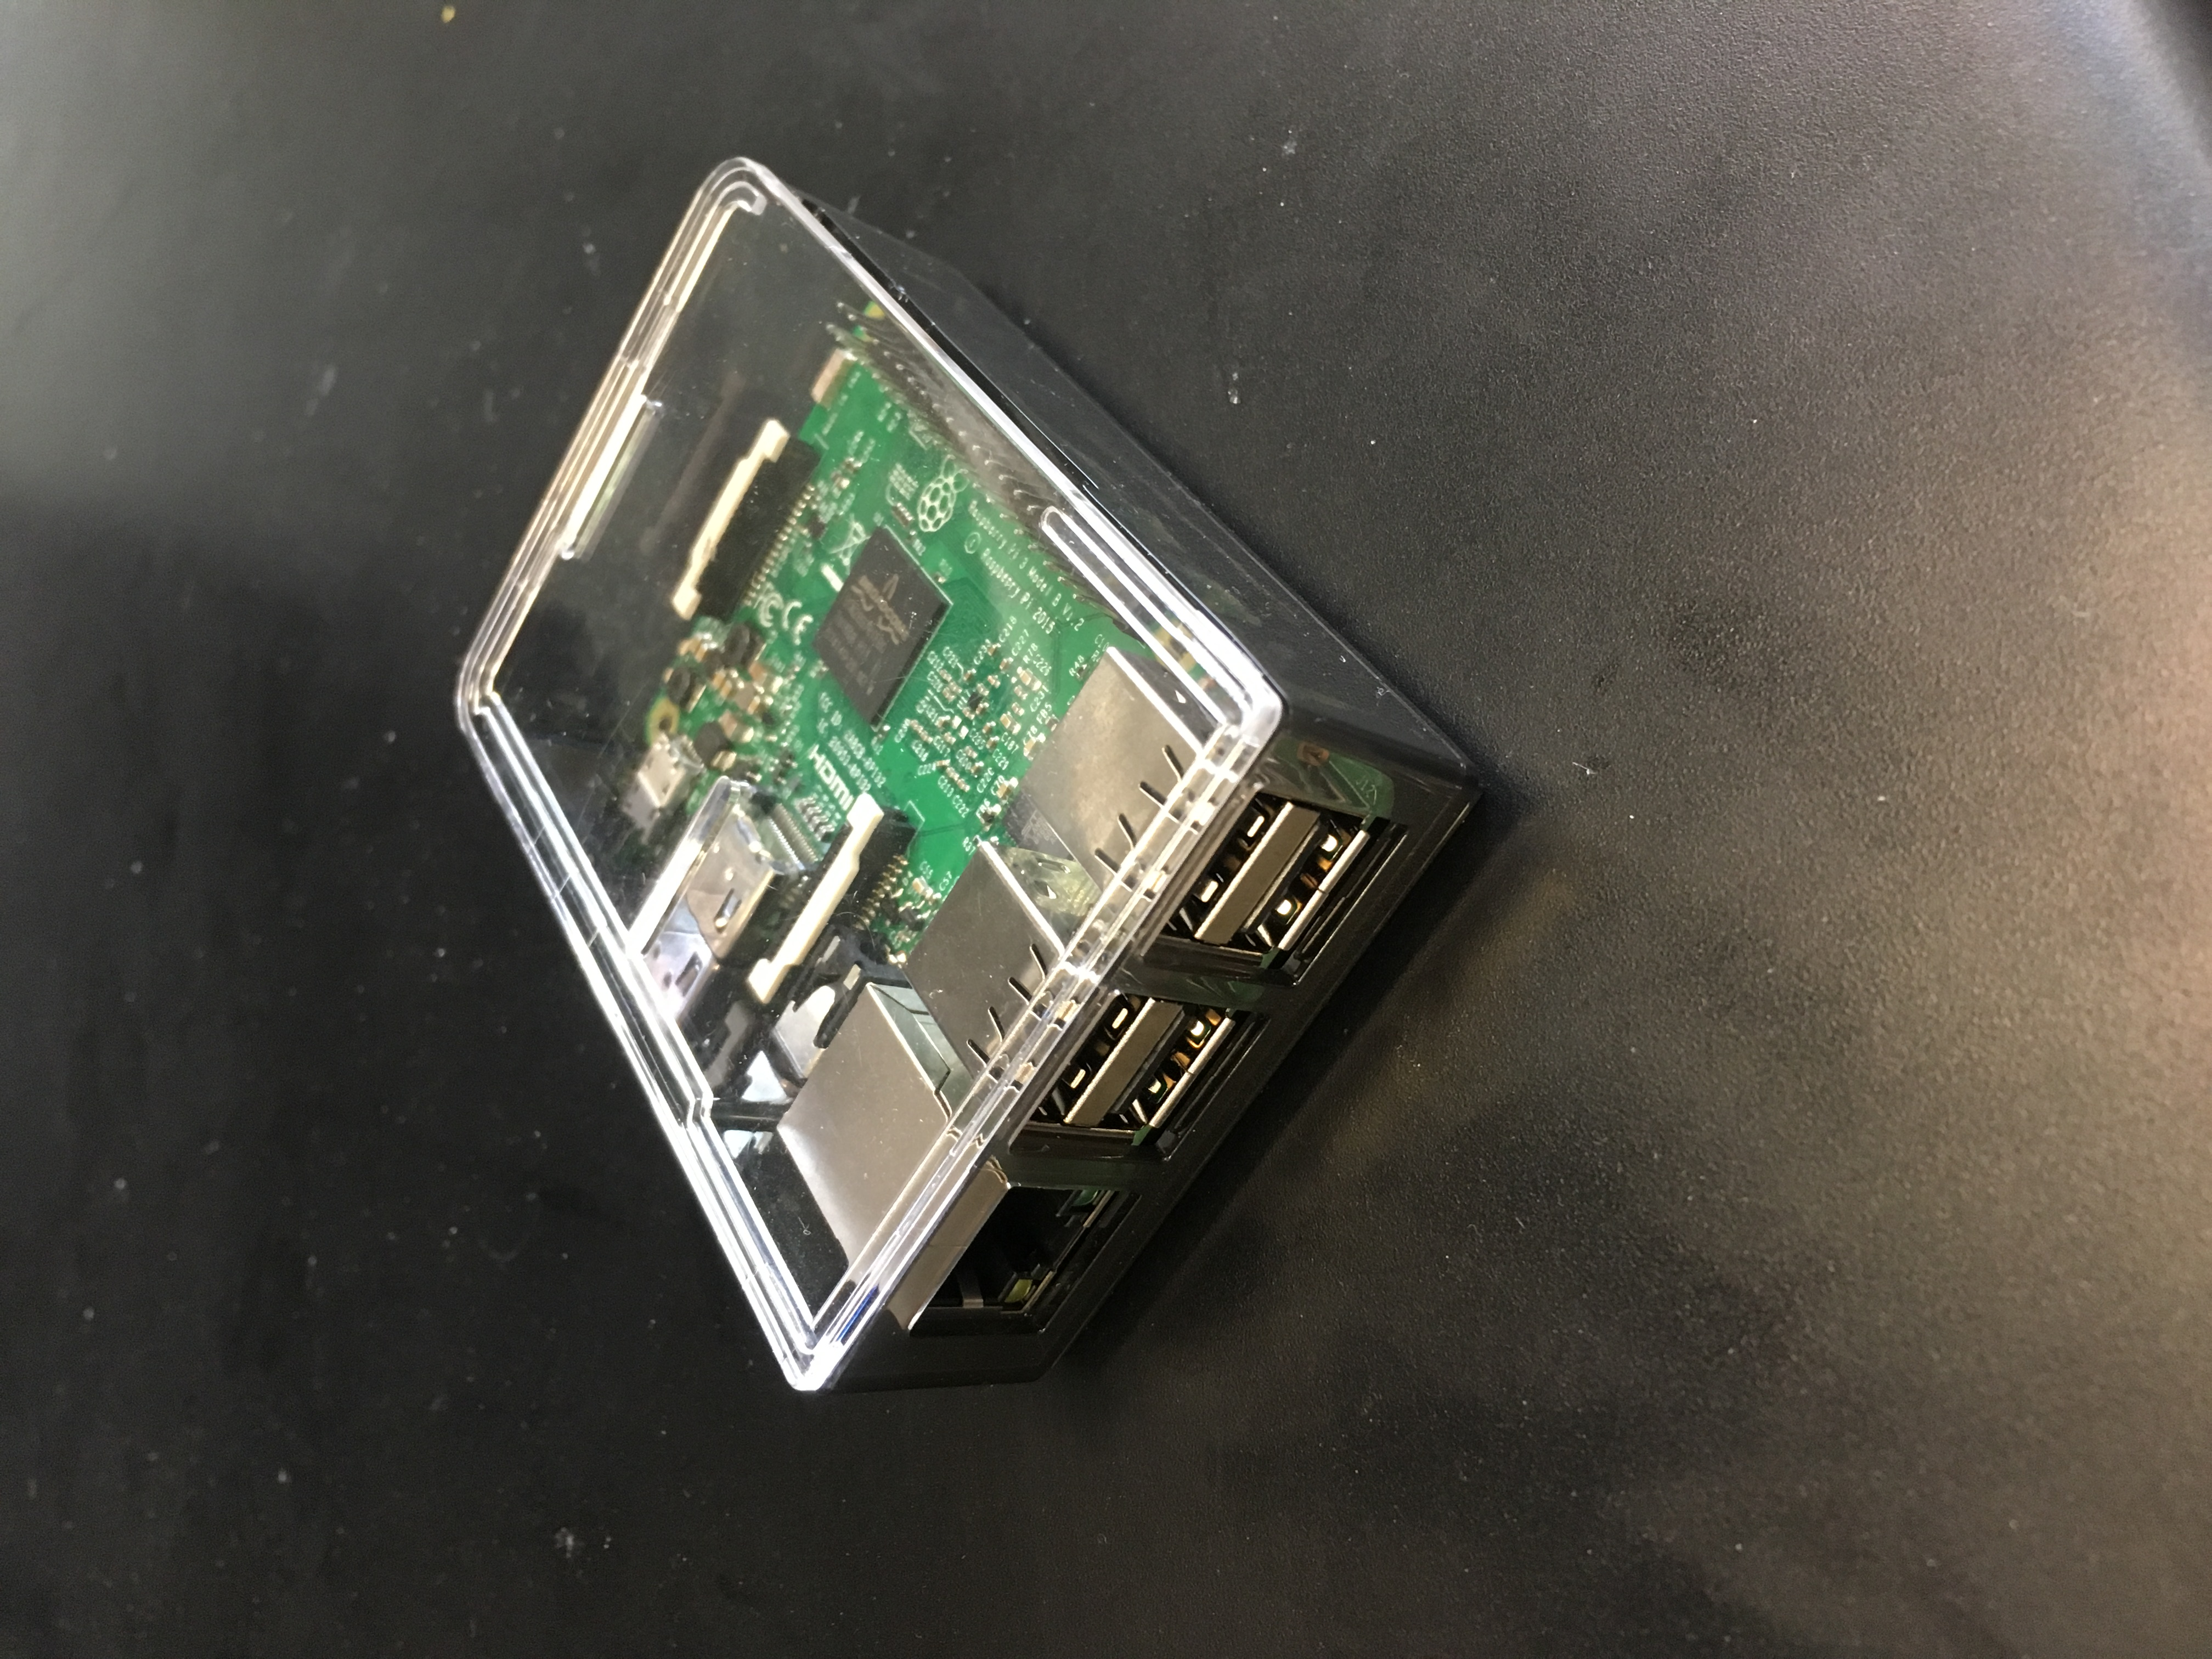
\includegraphics[width=\textwidth]{./figures//IMG_0708.JPG}
    \caption{Raspberry 2 (Raspberry Pi 3)}
    \label{fig:r2}
  \end{subfigure}
  \label{fig:rr}
\end{figure*}

The Powerchords are displayed below, first one showing a USB socket and the second one showing the usual chord.

\begin{figure*}[t]
  \centering
  \begin{subfigure}{.5\textwidth}
    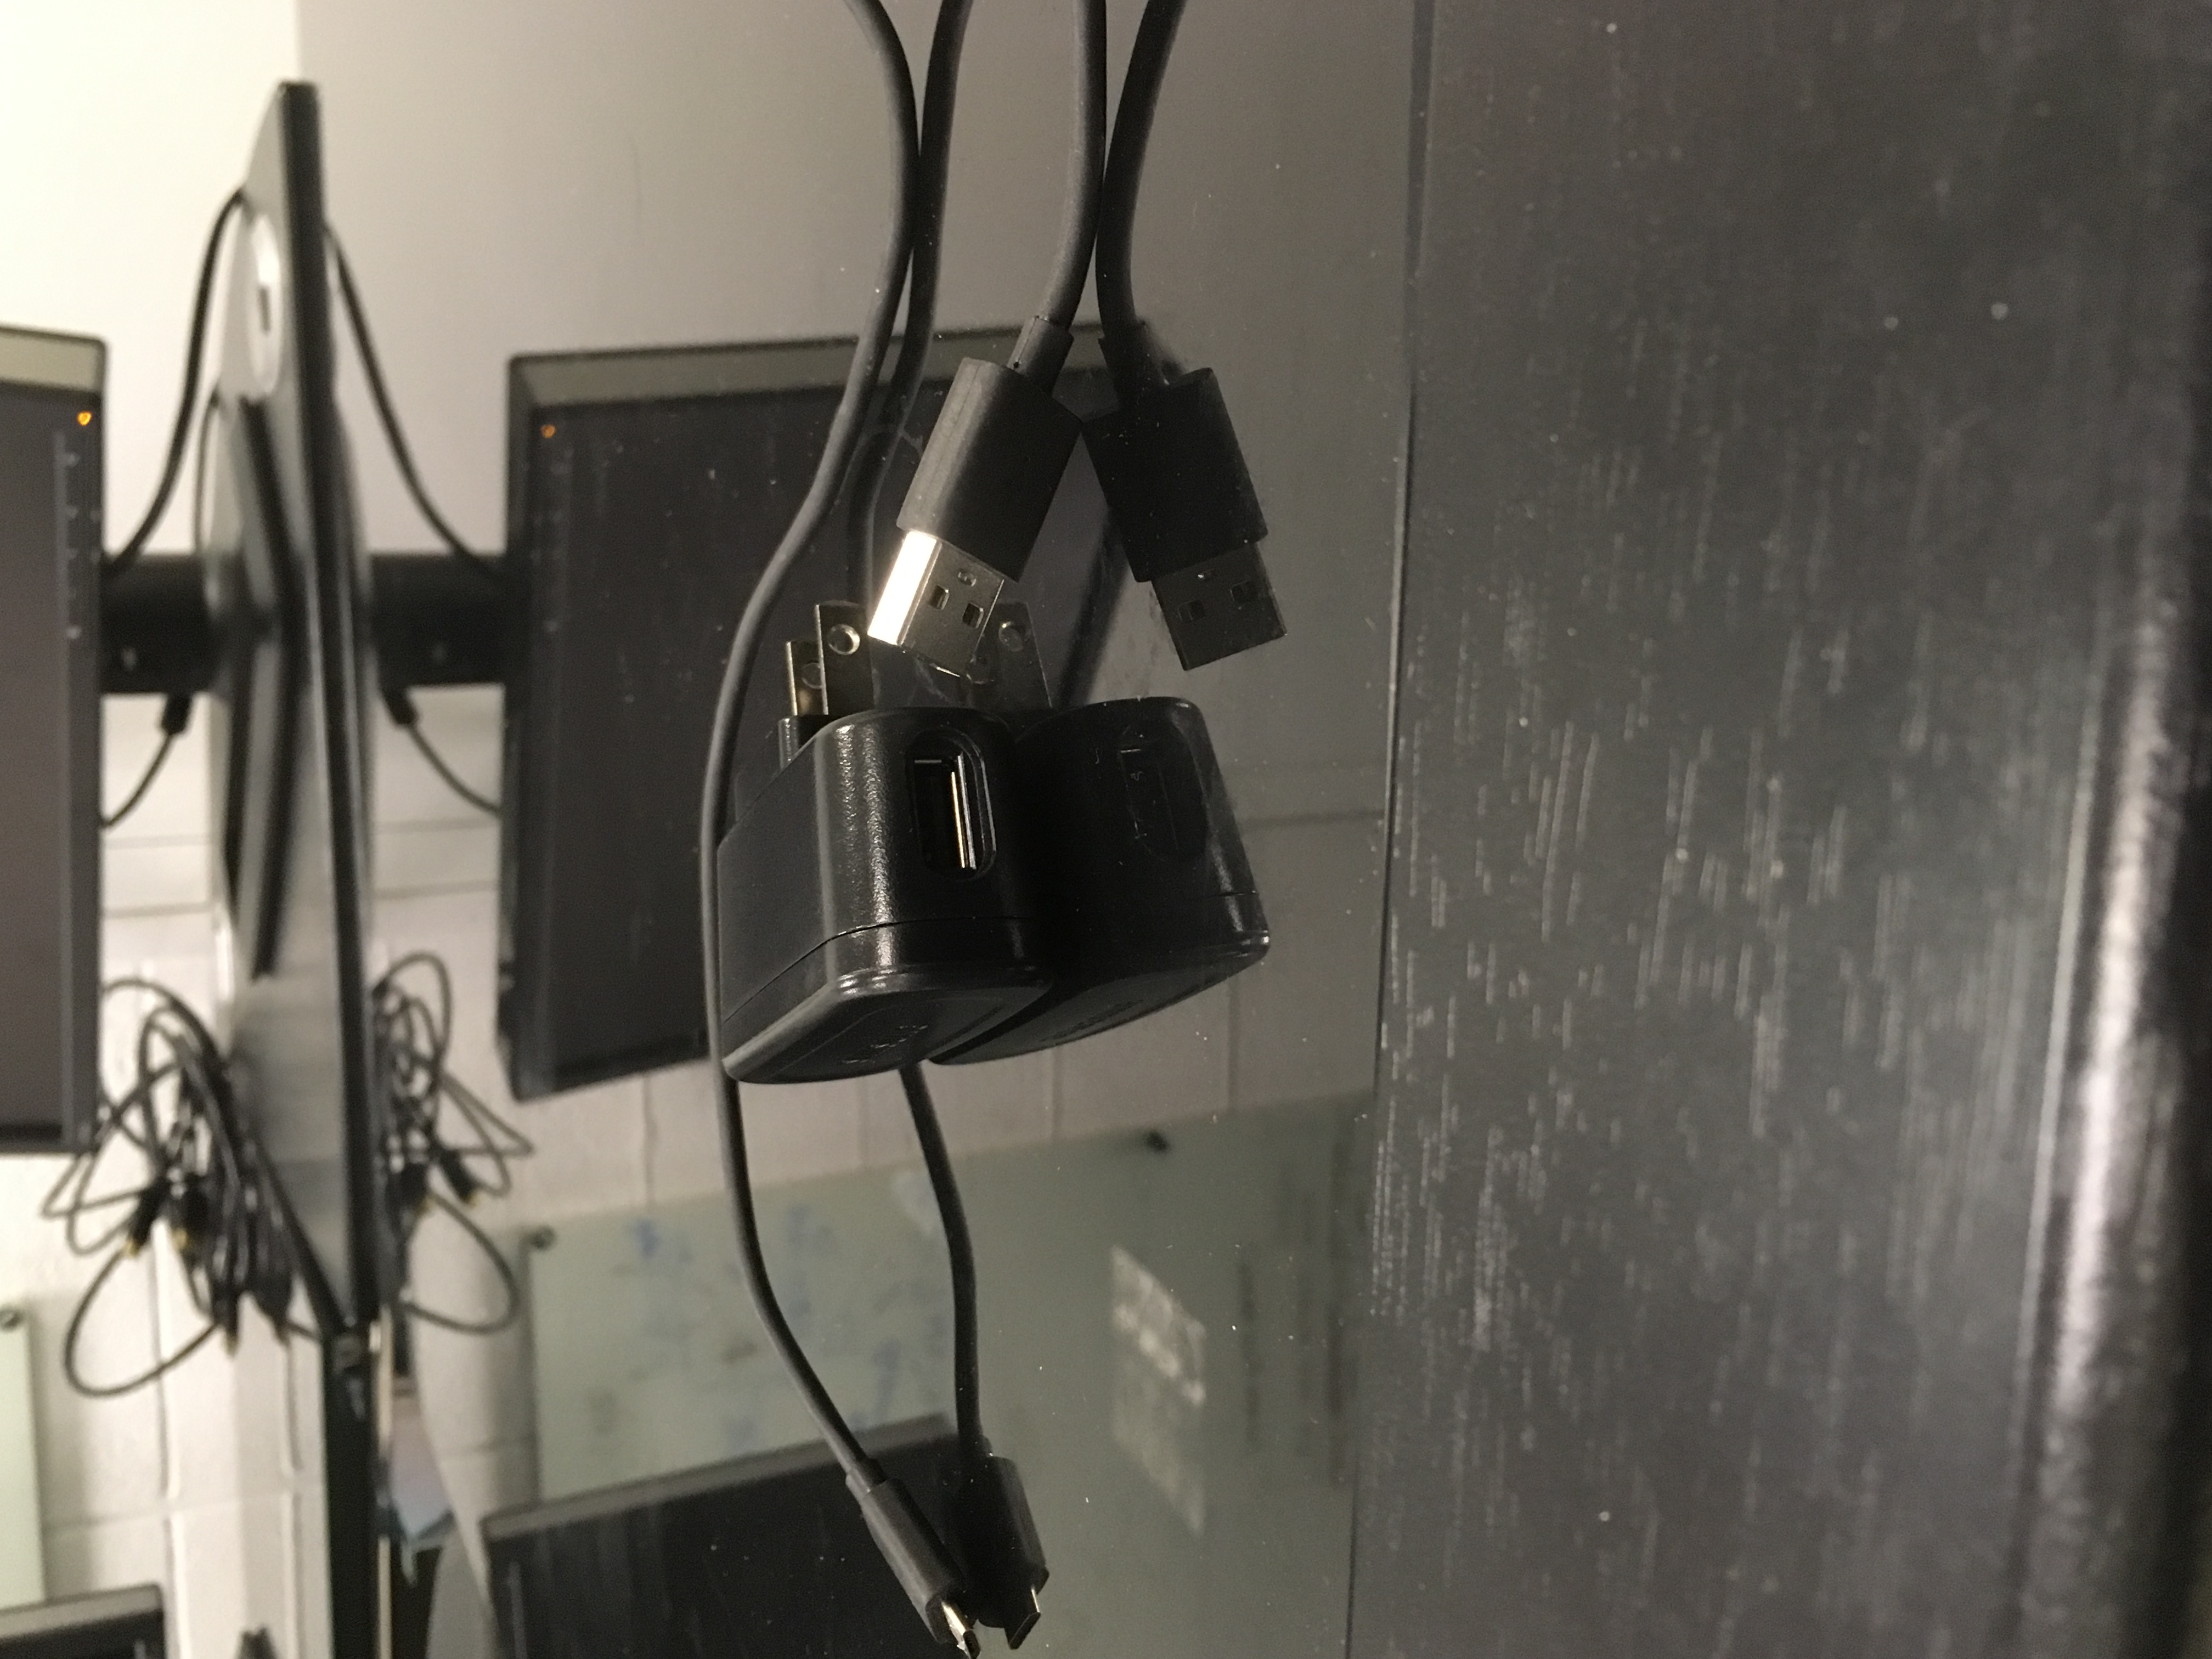
\includegraphics[angle=-90,width=\textwidth]{./figures//IMG_0712.JPG}
    \caption{Powerchord 1}
    \label{fig:p1}
  \end{subfigure}\hfill% 
  \centering
  \begin{subfigure}{.5\textwidth}
    \centering
    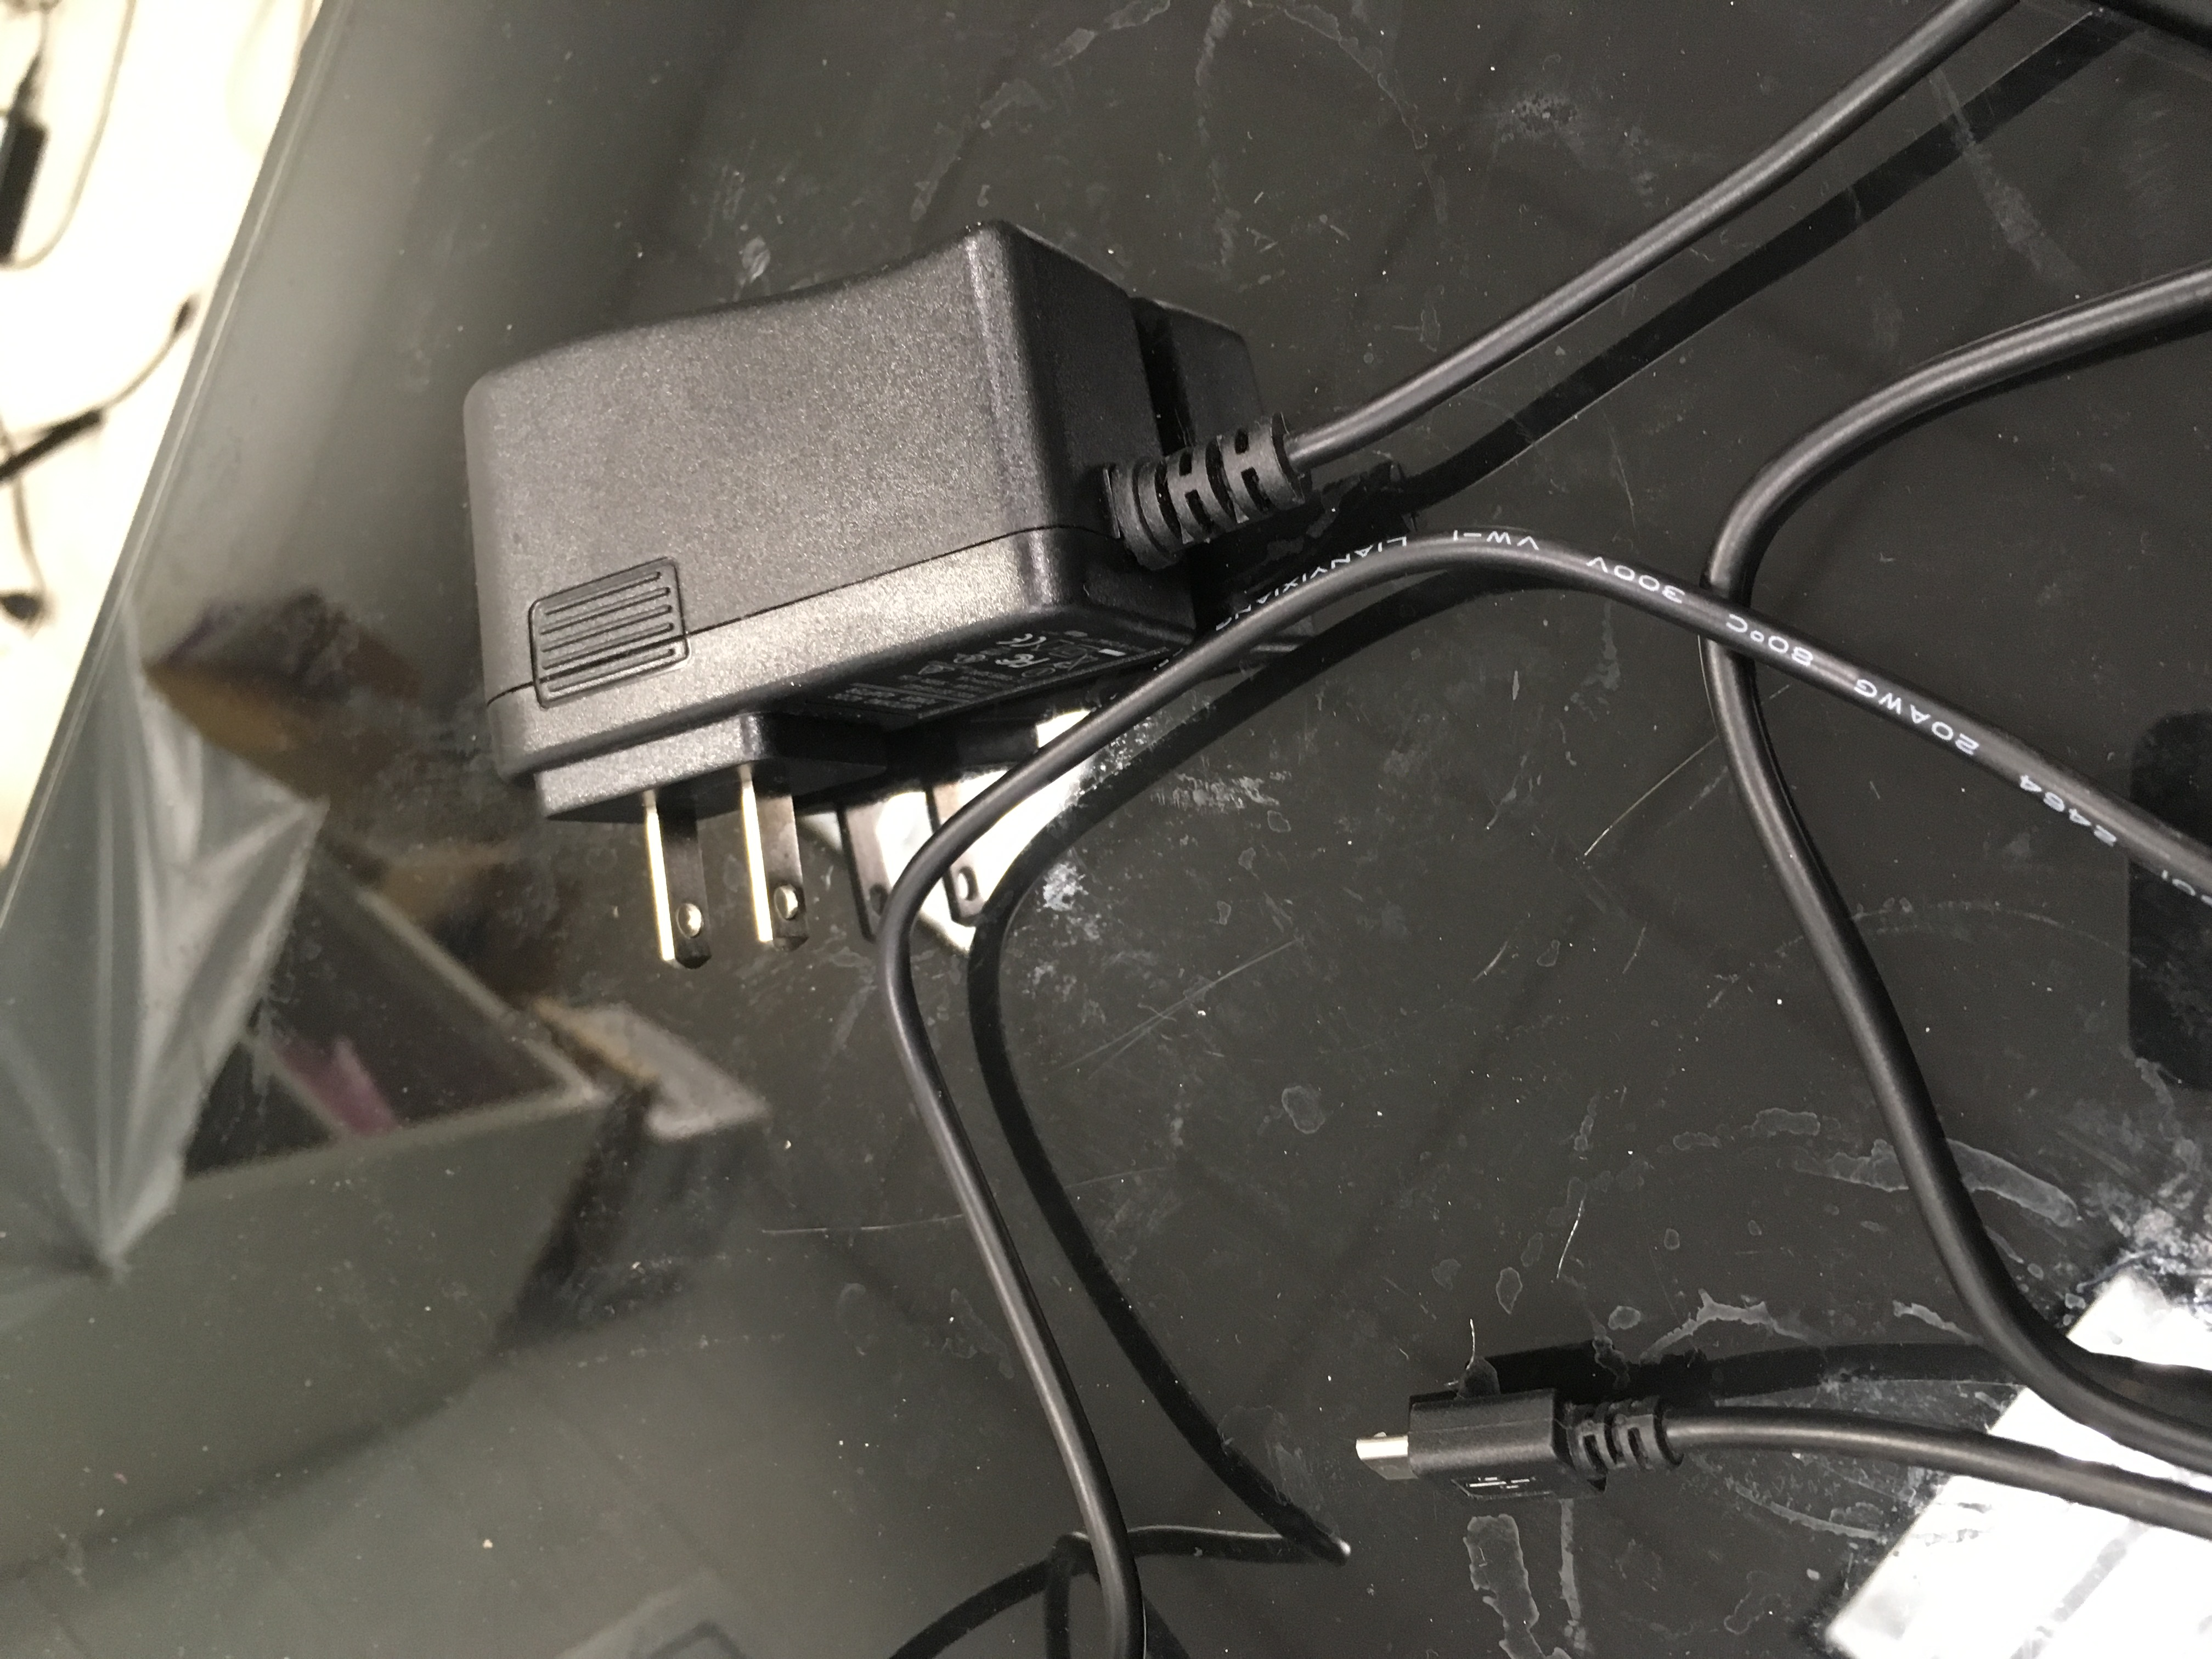
\includegraphics[angle=-90, width=\textwidth]{./figures//IMG_0710.JPG}
    \caption{Powerchord 2}
    \label{fig:p2}
  \end{subfigure}
  \label{fig:pp}
\end{figure*}

\end{document}
